\documentclass{article}
\usepackage{amsmath}
\usepackage{amsthm}
\usepackage{graphicx}
\usepackage{tikz}
\usepackage{pgfplots}
\usepackage{booktabs}
\usepackage{enumitem}
\usepackage[margin=1in]{geometry}
\usepackage{titlesec}

\titleformat{\section}[block]{\normalfont\large\bfseries\centering}{\thesection}{1em}{}
\titleformat{\subsection}[block]{\normalfont\bfseries\centering}{\thesubsection}{1em}{}

\theoremstyle{definition}
\newtheorem{definition}{Definition}
\newtheorem{example}{Example}

\title{Study Notes: Chapter 2 - Describing Data with Numerical Measures}
\author{Professor and Academic Researcher}
\date{}

\begin{document}
	
	\maketitle
	
	\section{Introduction to Chapter 2}
	
	Chapter 2 focuses on numerical descriptive statistics — summarizing quantitative data using measures of center, variability, relative standing, and graphical tools like box plots. These tools complement Chapter 1's graphical descriptions and are essential for understanding data distributions before proceeding to probability and inference.
	
	Key goal: Describe the central tendency, spread, and shape of a data set using numbers.
	
	\section{2.1 Measures of Center}
	
	\subsection{Key Measures}
	
	\begin{definition}[Arithmetic Mean (Average)]
		The sum of all measurements divided by the number of measurements.
	\end{definition}
	
	Population mean: \(\mu = \frac{\sum x_i}{N}\)
	
	Sample mean: \(\bar{x} = \frac{\sum x_i}{n}\)
	
	\begin{definition}[Median]
		The middle value when data are ordered. For \(n\) observations:
		- Odd \(n\): middle value
		- Even \(n\): average of two middle values
		Position: \((n+1)/2\)
	\end{definition}
	
	\begin{definition}[Mode]
		The value that occurs most frequently. May be none, one, or multiple.
	\end{definition}
	
	Detailed Explanation: 
	- Mean is sensitive to extreme values (skewed by outliers).
	- Median is resistant to outliers → preferred for skewed data.
	- Mode is useful for categorical or multimodal data.
	
	\begin{example}[Effect of Outliers]
		Data: 1, 2, 3, 4, 5 → mean = 3, median = 3
		
		Add outlier 100: mean = 23, median = 3.5 → median more stable.
	\end{example}
	
	\section{2.2 Measures of Variability}
	
	\subsection{Key Measures}
	
	\begin{definition}[Range]
		\(R = \max - \min\)
		Simple but sensitive to outliers.
	\end{definition}
	
	\begin{definition}[Variance]
		Average squared deviation from the mean.
		Population: \(\sigma^2 = \frac{\sum (x_i - \mu)^2}{N}\)
		
		Sample: \(s^2 = \frac{\sum (x_i - \bar{x})^2}{n-1}\) (unbiased estimator)
	\end{definition}
	
	\begin{definition}[Standard Deviation]
		Square root of variance: \(s = \sqrt{s^2}\)
		Has same units as data.
	\end{definition}
	
	Detailed Explanation: 
	- Variance measures spread in squared units.
	- Standard deviation is interpretable in original units.
	- Divisor \(n-1\) corrects bias in sample variance.
	
	\begin{example}[Computing Variance]
		Data: 2, 4, 6, 8 (\(\bar{x} = 5\))
		
		Deviations: -3, -1, 1, 3
		
		Squared: 9, 1, 1, 9 → sum = 20
		
		\(s^2 = 20 / 3 = 6.667\), \(s \approx 2.58\)
	\end{example}
	
	\section{2.3 Understanding and Interpreting the Standard Deviation}
	
	\subsection{Tchebysheff’s Theorem}
	
	For any distribution (regardless of shape):
	
	At least \(1 - 1/k^2\) of measurements lie within \(k\) standard deviations of the mean (\(k > 1\)).
	
	Examples:
	- \(k=2\): at least 75\% within \(\bar{x} \pm 2s\)
	- \(k=3\): at least 89\% within \(\bar{x} \pm 3s\)
	
	\subsection{Empirical Rule (Normal Distribution)}
	
	For mound-shaped, roughly symmetric data:
	
	- $\approx$ 68\% within \(\bar{x} \pm s\)
	- $\approx$ 95\% within \(\bar{x} \pm 2s\)
	- $\approx$ 99.7\% within \(\bar{x} \pm 3s\)
	
	\subsection{Approximating \(s\) Using the Range}
	
	Rough estimate: \(s \approx \frac{\text{range}}{4}\) (for moderate n and mound-shaped data).
	
	\begin{example}[Empirical Rule Application]
		Test scores: \(\bar{x} = 75\), \(s = 8\)
		
		$\approx$ 95\% /text{between} 59 and 91.
	\end{example}
	
	\section{2.4 Measures of Relative Standing}
	
	\subsection{z-Scores}
	
	Measures how many standard deviations a value is from the mean.
	
	\(z = \frac{x - \bar{x}}{s}\) (sample)
	
	\(z = \frac{x - \mu}{\sigma}\) (population)
	
	Interpretation: z = 1.5 → 1.5 SD above mean.
	
	\subsection{Percentiles and Quartiles}
	
	pth percentile: value below which p\% of observations fall.
	
	Position: \(p/100 \times (n+1)\)
	
	Quartiles:
	- Q1 (25th percentile)
	- Q2 = median
	- Q3 (75th percentile)
	
	Interquartile Range: IQR = Q3 – Q1
	
	\subsection{Five-Number Summary and Box Plot}
	
	Five-number summary: Min, Q1, Median, Q3, Max
	
	Box plot construction:
	- Box from Q1 to Q3
	- Median line inside box
	- Whiskers to min/max (or to 1.5 × IQR fences for outliers)
	
	Outliers: values beyond Q1 – 1.5 IQR or Q3 + 1.5 IQR
	
	\begin{example}[Box Plot Interpretation]
		Skewed right data: longer upper whisker, median closer to Q1.
	\end{example}
	
	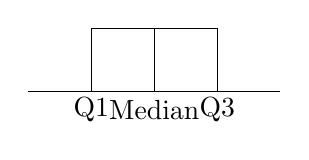
\begin{tikzpicture}[scale=0.8]
		% Simple box plot example
		\draw (0,0) -- (4,0);
		\draw (1,0) rectangle (3,1);
		\draw (2,0) -- (2,1);
		\draw (0.5,0.5) -- (0.5,0.5); % lower whisker
		\draw (3.5,0.5) -- (3.5,0.5); % upper whisker
		\node at (2,-0.3) {Median};
		\node at (1,-0.3) {Q1};
		\node at (3,-0.3) {Q3};
	\end{tikzpicture}
	
	\section{Chapter Review}
	
	Key concepts:
	- Center: mean, median, mode
	- Variability: range, variance, standard deviation
	- Relative position: z-scores, percentiles, quartiles
	- Distribution shape \& outliers: box plots, Empirical Rule, Tchebysheff’s Theorem
	
	Formulas summary:
	- \(\bar{x} = \frac{\sum x_i}{n}\)
	- \(s^2 = \frac{\sum (x_i - \bar{x})^2}{n-1}\)
	- \(z = \frac{x - \bar{x}}{s}\)
	- IQR = Q3 – Q1
	
	\section{Technology Today}
	
	Use calculators/software (TI-84, Excel, MINITAB) for:
	- 1-Var Stats → mean, median, s, five-number summary
	- Box plots and outlier detection
	
	\section{Case Study: The Boys of Summer}
	
	Analyze baseball data (e.g., batting averages, home runs) using measures of center and variability to compare performance across eras or teams.
	
\end{document}